 \chapter{Resultados}
\label{cap:resultados}

O objetivo geral deste trabalho foi plenamente alcançado com a criação de uma plataforma digital que une um site moderno e um ambiente virtual 3D, ambos voltados para a preservação, divulgação e democratização do acesso à arte rupestre da cidade de Formosa, Goiás. O novo site apresenta um design responsivo, organização clara das informações e funcionalidades como galeria de imagens e acesso a modelos 3D, enquanto o ambiente virtual proporciona uma imersão detalhada nas pinturas rupestres, permitindo exploração interativa e download para uso offline. Essa solução não apenas resolve os problemas de usabilidade e acessibilidade identificados no site anterior, mas também promove a conscientização sobre a importância desses registros culturais, alinhando-se ao propósito de preservar e valorizar o patrimônio arqueológico da região de Formosa.
As seções a seguir detalham como os objetivos específicos foram atendidos.

\s\ection{Análise Heurística de Usabilidade: Problemas Identificados no Site Antigo}
Um dos objetivos específicos era realizar uma análise heurística de usabilidade do antigo site "Arqueologia Formosa". Essa análise foi conduzida com base nas heurísticas de Nielsen, avaliando aspectos como navegabilidade, eficiência e consistência. Os principais problemas identificados foram:
\begin{itemize}
    \item Layout desorganizado, dificultando a localização de informações importantes.
    \item Falta de responsividade para dispositivos móveis.
    \item Ausência de funcionalidades modernas, como busca por filtros e visualização do modelo 3D dentro do próprio site.
\end{itemize}

Esses problemas foram utilizados como base para o planejamento do novo site, garantindo que as falhas do sistema anterior fossem corrigidas. A análise heurística também guiou a priorização das melhorias implementadas.

\section{Implementação de um Ambiente Virtual \gls{3d}}
Outro objetivo específico era implementar um ambiente virtual \gls{3d} que permitisse a visualização interativa da arte rupestre. Esse objetivo foi alcançado com o desenvolvimento de um ambiente imersivo na Unreal Engine, utilizando modelos \gls{3d} gerados por fotogrametria. Os resultados incluem:
\begin{itemize}
    \item Fidelidade visual dos modelos \gls{3d} gerados por fotogrametria, com texturas realistas das pinturas rupestres;
    \item Navegação interativa no ambiente, permitindo aos usuários explorar o sítio arqueológico em primeira e terceira pessoa;
    \item Avatar personalizado baseado no professor Edson Borges;
    \item Empacotamento do ambiente virtual em um arquivo executável, disponibilizado para \textit{download} no site.
\end{itemize}

A Figura \ref{fig:virtual_environment} apresenta uma visão do ambiente virtual desenvolvido.

\begin{figure}[H]
    \centering
    % Substitua pelo caminho do arquivo de imagem
    \includegraphics[width=0.8\linewidth]{img/unreal/mapa.png}
    \caption{Ambiente virtual desenvolvido na Unreal Engine.}
    \label{fig:virtual_environment}
\end{figure}

\section{Desenvolvimento de um Novo Site com Design Centrado no Usuário (\gls{ux})}
O novo site foi desenvolvido com tecnologias modernas (\textit{Next.js}, \textit{Tailwind CSS} e \textit{Sanity CMS}), priorizando uma experiência do usuário intuitiva e acessível. Os resultados alcançados incluem:
\begin{itemize}
    \item Design responsivo, otimizado para dispositivos móveis, desktops e tablets.
    \item Galeria de imagens organizada, com suporte para visualização ampliada.
    \item Modo escuro/claro, permitindo maior conforto visual.
    \item Implementação de padrões de acessibilidade conforme WCAG 2.1 (nível AA).
\end{itemize}

A Figura \ref{fig:site_homepage} apresenta a página inicial do novo site, evidenciando o layout moderno e a organização do conteúdo.

\begin{figure}[H]
    \centering
    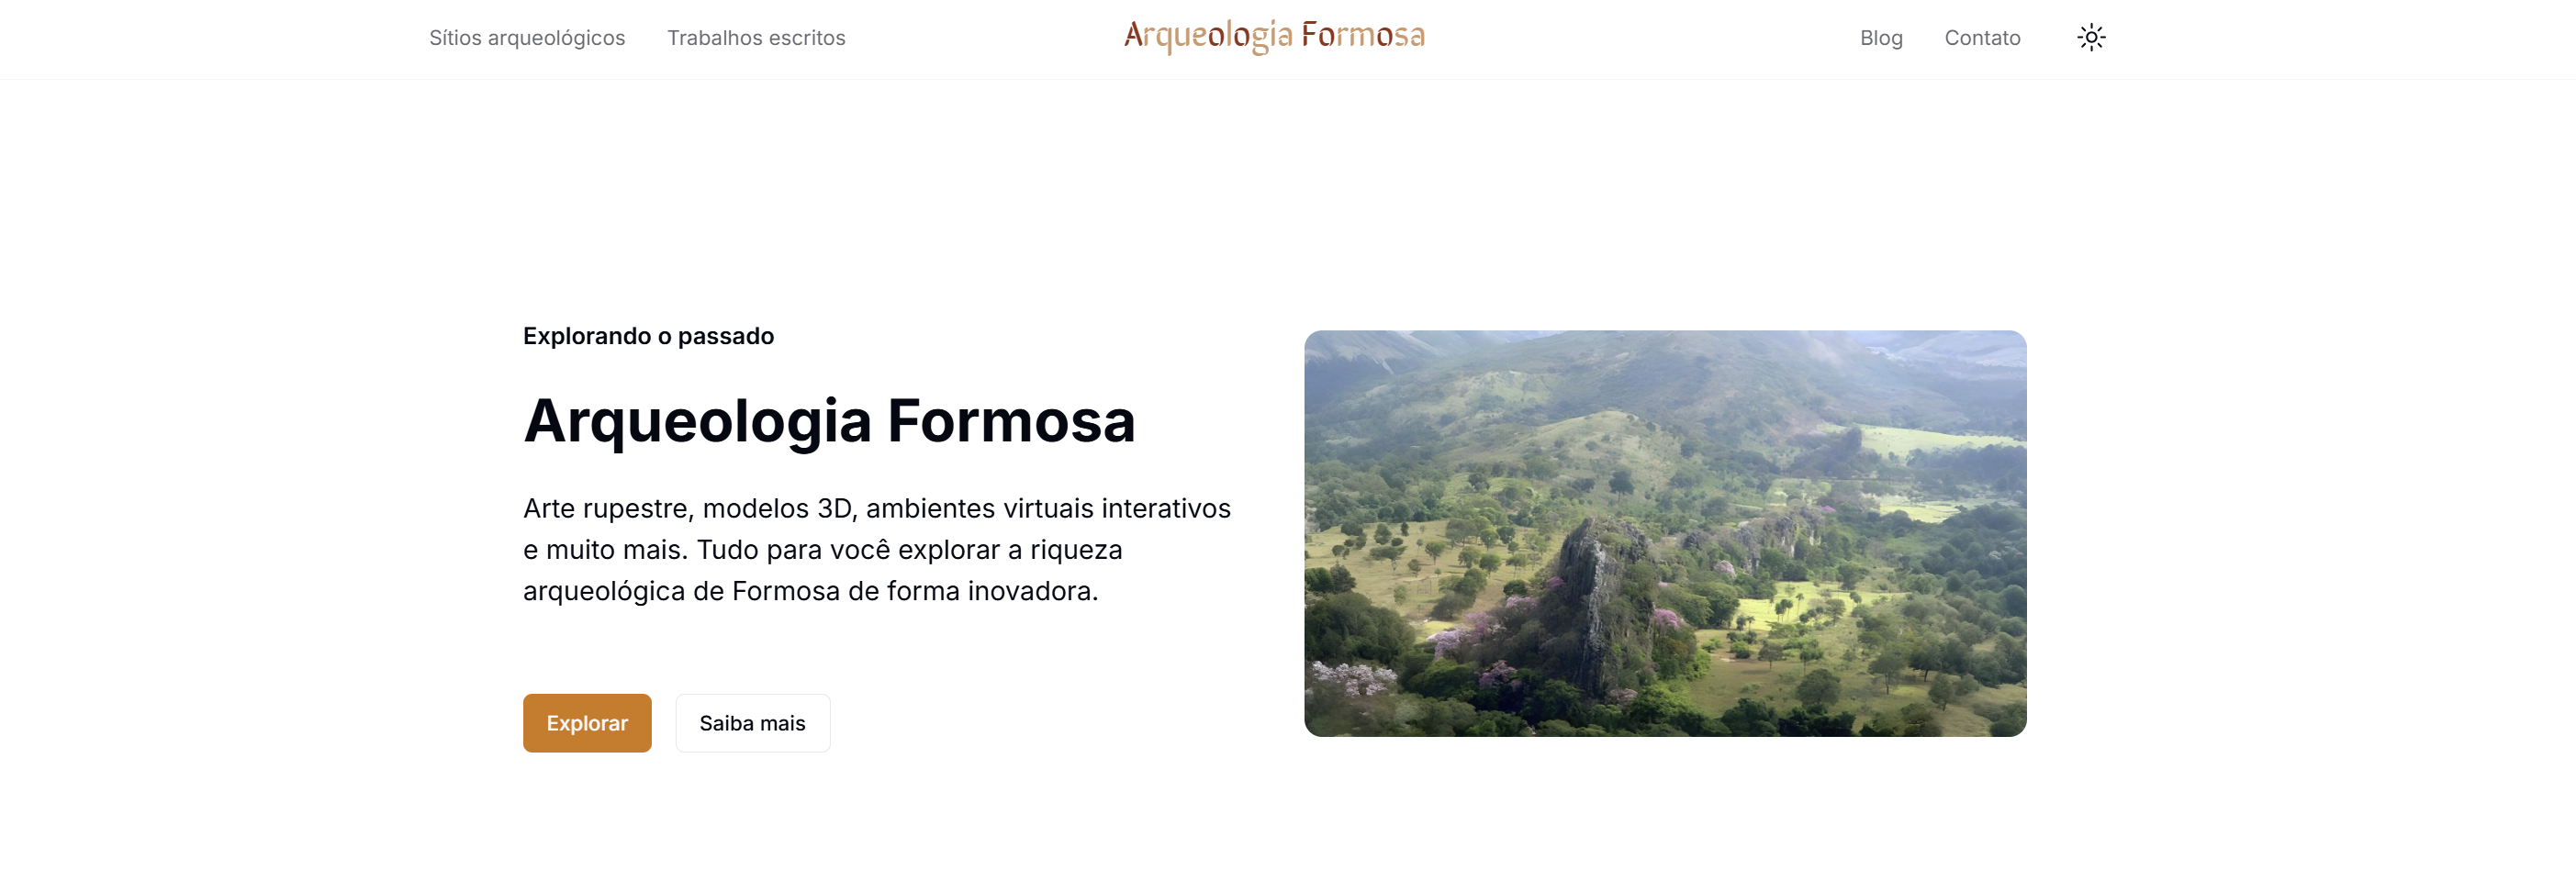
\includegraphics[height=6cm, keepaspectratio]{img/site/hero1.png}
    \caption{Página inicial do novo site "Arqueologia Formosa". \\
    \textbf{Fonte:} Elaborado pelo autor, 2025.}
    \label{fig:site_homepage}
\end{figure}

As demais páginas podem ser vista no Apêndice \ref{ap:páginas_do_site} e no site publicado na internet, acessível por meio do endereço \url{www.arqueologiaformosa.com.br}.

\section{Testes e Validação}
Para comprovar a qualidade do produto desenvovido foram realizados alguns testes. Os resultados desses testes estão descritos abaixo:
% \subsection{Usabilidade}
% Os testes de usabilidade foram realizados com base nas heurísticas de Nielsen. Os seguintes pontos foram avaliados:
% \begin{itemize}
%     \item Facilidade de navegação no site e no ambiente virtual.
%     \item Eficiência na interação com a galeria de imagens e o ambiente virtual.
%     \item Satisfação dos usuários com o design e as funcionalidades implementadas.
% \end{itemize}


% \begin{table}[H]
% \centering
% \caption{Resultados dos testes de usabilidade.}
% \label{tab:usabilidade}
% \begin{tabularx}{\textwidth}{|l|X|X|} % Ajusta a largura da tabela ao texto
% \hline
% \textbf{Critério Avaliado} & \textbf{Pontuação Média} & \textbf{Observações} \\ \hline
% Facilidade de Navegação    & 4.7/5                   & Navegação intuitiva e bem estruturada. \\ \hline
% Interação com o Conteúdo    & 4.6/5                   & Boa experiência na galeria de imagens e no ambiente virtual. \\ \hline
% Design e Funcionalidades    & 4.8/5                   & Alta satisfação com o layout moderno e intuitivo. \\ \hline
% \end{tabularx}
% \end{table}
\begin{enumerate}

\item{Desempenho}
Os testes de desempenho foram realizados com o \textit{Google Lighthouse}. Abaixo estão os principais resultados:
\begin{table}[H]
\centering
\caption{Resultados dos testes de desempenho realizados com o \textit{Google Lighthouse}.}
\label{tab:desempenho}
\begin{tabularx}{\textwidth}{|l|X|} % Ajusta a largura da tabela ao texto
\hline
\textbf{Critério Avaliado} & \textbf{Resultado} \\ \hline
Tempo de carregamento médio & 1 segundo \\ \hline
Tempo até o primeiro conteúdo visível aparecer & 0,8 segundos \\ \hline
Pontuação em SEO & 100/100 \\ \hline
Pontuação em Desempenho & 95/100 \\ \hline
Responsividade & Boa responsividade em dispositivos móveis e desktops \\ \hline
\end{tabularx}
\end{table}
As Figuras \ref{fig:lighthouse} e \ref{fig:tempocarregamento} mostram capturas de tela dos testes realizados com a ferramenta \textit{Google Lighthouse}.
\begin{figure}[H]
    \centering
    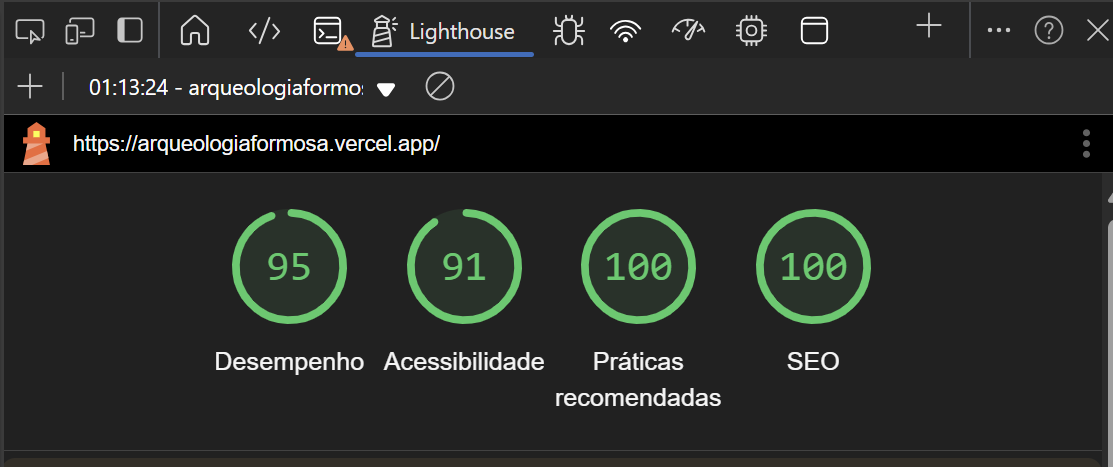
\includegraphics[height=6cm, keepaspectratio]{img/site/lighthouse_only.png}
    \caption{Análise de desempenho do site Arqueologia Formosa pela ferramenta \textit{Lighthouse}. \\
    \textbf{Fonte:} Elaborado pelo autor, 2025.}
    \label{fig:lighthouse}
\end{figure}

\begin{figure}[H]
    \centering
    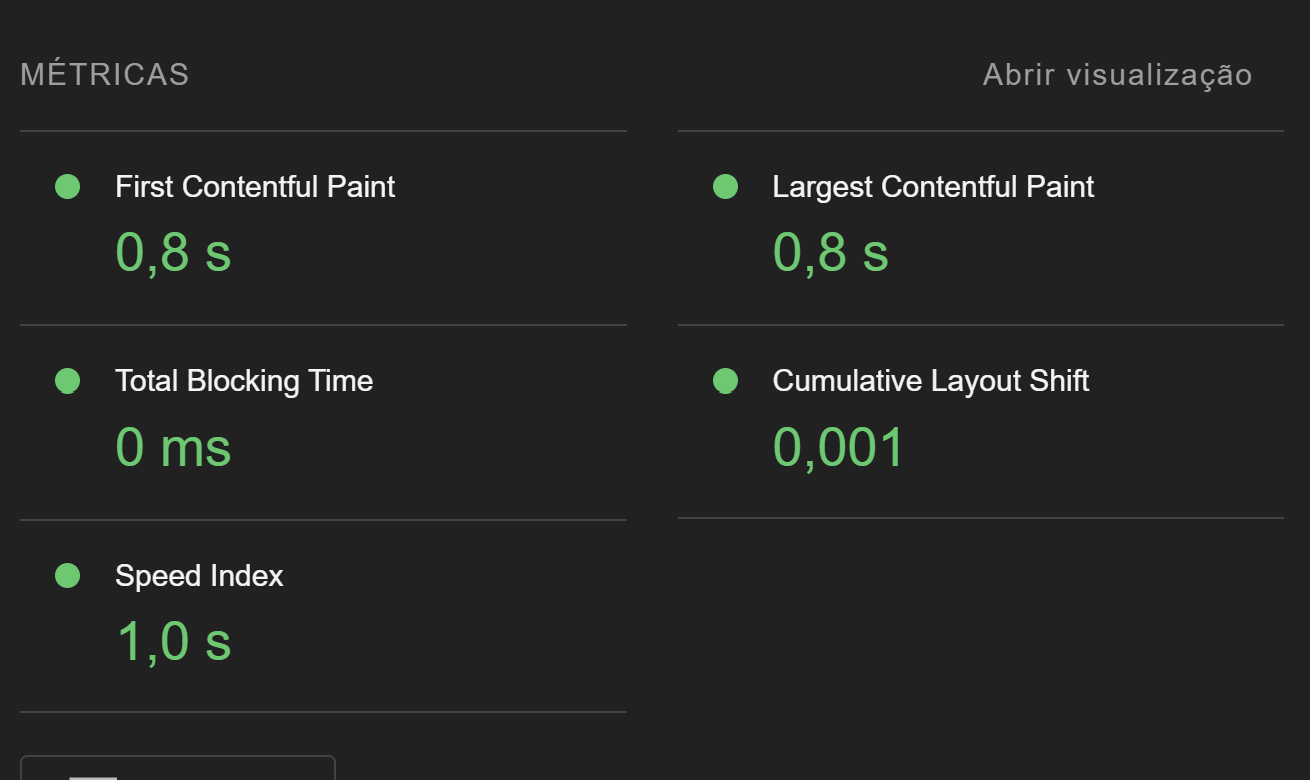
\includegraphics[height=6cm, keepaspectratio]{img/site/tempo_de_carregamento.png}
    \caption{Tempo de carregamento da página medido pelo \textit{Lighthouse}. \\
    \textbf{Fonte:} Elaborado pelo autor, 2025.}
    \label{fig:tempocarregamento}
\end{figure}

\item{Acessibilidade}
O site final seguiu as regras de conformidade com as diretrizes WCAG 2.1, e foram medidas com testes de usabilidade e teste de contraste feitas no site \href{https://dequeuniversity.com/rules/axe/4.10/color-contrast}{\textit{Deque University - Color Contrast}}. Foram garantidos o contraste adequado para textos e botões (Figura \ref{fig:testeconstraste}); a navegação por teclado funcionando corretamente; e a compatibilidade com leitores de tela. O leitor de tela utilizado para os testes foi o \href{https://www.tcees.tc.br/acessibilidade/leitor-de-tela-nvda/}{NVDA}\footnote{NVDA é um programa de código aberto para leitura de tela que permite que pessoas cegas ou com deficiência visual acessem e interajam com o sistema através de voz sintética.}. Além disso o site alcançou uma pontuação de 91/100 em acessibilidade utilizando a ferramenta \textit{Lighthouse}, como mostrado na Figura \ref{fig:lighthouse}

\begin{figure}[H]
    \centering
    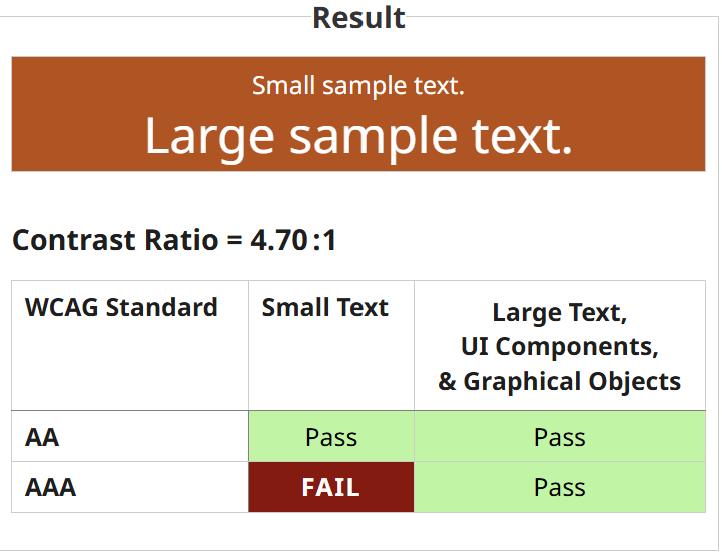
\includegraphics[height=6cm, keepaspectratio]{img/site/contraste.png}
    \caption{Teste de constraste de acordo com o \\ padrão WCAG medido pela ferramenta de contraste da \href{https://dequeuniversity.com/rules/axe/4.10/color-contrast}{\textit{Deque University}}. \\
    \textbf{Fonte:} Elaborado pelo autor, 2025.}
    \label{fig:testeconstraste}
\end{figure}

\end{enumerate}

